%!TEX root = ./template-skripsi.tex
%-------------------------------------------------------------------------------
% 								BAB I
% 							LATAR BELAKANG
%-------------------------------------------------------------------------------

\chapter{LATAR BELAKANG}

\section{Latar Belakang Masalah}
Setiap hari semua manusia di dunia, tanpa terkecuali, membutuhkan makanan untuk dikonsumsi. Manusia mengonsumsi makanan setiap harinya untuk memenuhi kebutuhan tubuh. Untuk dapat beraktifitas normal, tubuh manusia membutuhkan energi. Energi tersebut didapat dari mengonsumsi makanan setiap harinya.

Orang-orang biasanya memasak sendiri makanan yang akan mereka konsumsi. Beragam alasan yang dimiliki orang-orang yang memilih memasak sendiri makanan yang hendak mereka konsumsi, mulai dari faktor kebersihan yang lebih terjamin, biaya yang lebih terjangkau, rasa yang lebih enak karena dapat dikontrol secara langsung, hobi memasak, mahir memasak, dan alasan lainnya. 

Meskipun banyak orang yang memilih memasak sendiri makanannya, tidak sedikit juga yang memilih untuk tidak memasak sendiri makanan yang hendak ia konsumsi. Bagi yang memiliki dana berlebih biasanya memilih membeli makanan yang hendak ia konsumsi karena praktis dan hemat waktu. Orang yang tidak tinggal bersama keluarganya, seperti mahasiswa yang sedang kuliah di luar kota atau karyawan yang sedang dinas di luar kota biasanya juga lebih memilih mengeluarkan uang untuk membeli makanan demi memenuhi kebutuhan energi untuk menjalankan aktifitas sehari-hari. Harga yang bervariasi serta rasa yang enak juga menjadi pertimbangan kebanyakan orang untuk tidak memasak makanannya sendiri.

Kendala utama yang dirasakan orang-orang pada umumnya saat memasak adalah hampir 90 persen masyarakat Indonesia disibukkan dengan pekerjaan, sehingga rasa lelah lebih mendera. Hal inilah yang membuat mereka enggan memasak. Semua orang memiliki kemampuan untuk memasak namun terkendala oleh waktu. Menghindari atau enggan membersihkan serta membereskan peralatan masak juga menjadi alasan mengapa orang-orang enggan memasak \cite{poernomo}.

Berdasarkan survei yang dilakukan oleh Fiesta Seafood terhadap perempuan berusia 25 - 45 tahun di lima kota, Jakarta, Depok, Bandung, Surabaya dan Yogyakarta, mengungkapkan bahwa ada tiga alasan utama yang membuat seseorang enggan memasak sendiri di rumah, yaitu kesibukan kerja dan urusan rumah tangga lainnya, tidak tahu bumbu, resep atau cara memasak untuk menghasilkan makanan yang enak, tak memiliki motivasi serta dukungan untuk memasak. 

Memasak identik dengan kegiatan mengupas, memotong, menumis, dan kegiatan yang tidak mudah lainnya. Padahal ada banyak makanan sederhana yang tidak sulit untuk dimasak. Seharusnya ini tak lagi jadi masalah, karena sekarang sudah ada internet yang dengan mudah membantu untuk belajar memasak \cite{poernomo}.

Perempuan yang sedianya dikenal sebagai kaum yang mahir memasak pun kini tidak lagi seluruhnya mahir memasak. Seiring waktu, tak bisa dipungkiri bahwa beragam aktivitas dan tuntutan pekerjaan membatasi ruang dan waktu perempuan. Alhasil, aktivitas memasak di rumah bukan lagi dipandang sebuah rutinitas. Masakan ibu pun tergantikan dengan ketersediaan pelayanan delivery makanan siap saji, layanan katering, atau makanan instan. Riset yang dilakukan \emph{Journal of Nutrition Education and Behaviour} yang diringkas oleh situs tabloidnova.com menemukan, 3 dari 4 ibu bekerja mengaku bahwa mereka tidak punya akses dan waktu untuk membuat makanan yang sehat dan bergizi di rumah. 

Bersamaan dengan itu, riset ini juga mengatakan bahwa sulitnya akses dan waktu untuk memasak di rumah yang banyak dialami para wanita bekerja, kerap menjadi faktor yang buruk. Di antaranya, cenderung memberi contoh pola makan yang tidak baik pada keluarga. Perlu disadari kembali, manfaat memasak di rumah memang tak ternilai pentingnya. Semakin sedikit waktu yang diluangkan secara konsisten bersama keluarga setiap hari, akan membuat anak-anak tumbuh kurang optimal, kurang rasa percaya diri, dan tidak peduli dengan kondisi lingkungan sekitar \cite{inirani}.

Masih menurut survei yang sama, ditemukan pula bahwa 9 dari 10 wanita sebenarnya ingin bisa memasak. Namun, mereka mengakui begitu banyak kendala yang dialami untuk kembali ke dapur. Kendala tersebut, menempati posisi pertama adalah karena tidak memiliki waktu, disusul tidak mempunyai ilmu dan pengetahuan dalam mengolah masakan, serta tidak adanya motivasi dan dukungan yang menyemangati untuk memasak.

Pada era globalisasi yang diliputi oleh kemajuan teknologi seperti sekarang ini, masyarakat Indonesia dimanjakan oleh berbagai macam kemudahan untuk dapat membeli makanan di restoran dan bahkan di warung sederhana sekalipun. Selain harus datang langsung ke restoran atau warung makan yang mereka tuju, kini orang-orang dapat juga memesan makanan tersebut untuk diantarkan ke alamat yang diinginkan oleh pemesan melalui telepon, aplikasi pada ponsel cerdas, dan melalui \emph{website} yang dikelola oleh restoran itu sendiri. 

Kemudahan-kemudahan yang disediakan tersebut mendorong masyarakat menjadi lebih konsumtif. Perilaku hidup yang konsumtif dapat menyebabkan pemborosan. Padahal, masyarakat yang memasak sendiri makanan yang dikonsumsinya secara otomatis telah berhemat dan mengurangi sifat konsumtif yang dimiliki oleh masing-masing individu. Selain itu, dengan memasak sendiri makanan yang hendak dikonsumsi, masyarakat mengetahui tingkat kebersihan makanan tersebut dan menambah wawasan seperti mengetahui banyak macam rempah-rempah yang bisa dijadikan bumbu makanan, mengetahui berbagai jenis sayur, ikan, daging, dan bahan makanan lainnya. Ketersediaan teknologi yang canggih seperti saat ini dapat mempermudah masyarakat Indonesia untuk belajar memasak sendiri di rumah dengan mencari resep masakan melalui mesin pencari Google. Orang-orang juga dapat langsung menonton cara memasak sebuah makanan dengan menggunakan YouTube dengan memilih saluran masak berbagai genre mulai dari koki rumahan, orang yang baru belajar memasak, hingga chef-chef ternama pemilik restoran berbintang. Memasak masakan berat dan rumit sampai hidangan ringan dan super mudah, seperti mug cake, yang selesai dimasak dalam 2 menit.

Oleh karena itu, peneliti memilih untuk mengembangkan sebuah aplikasi resep masakan pada \textit{smartphone} berbasis Android. Terdapat berbagai alasan yang dipertimbangkan oleh penulis mengenai pemilihan \textit{platform} Android ini karena Android bukanlah satu-satunya sistem operasi yang terdapat pada ponsel cerdas saat ini. iOS, BlackBerry OS, dan Windows Phone merupakan sistem operasi yang menjadi pesaing ketat Android di pasar. Seperti yang dikutip dari situs Android Authority, terdapat beberapa alasan masyarakat dunia menggunakan ponsel berbasis Android yaitu:
\begin{enumerate}
	\item Harga yang menyesuaikan dengan kebutuhan\\
	Dengan dana yang terbatas sekalipun anda dapat merasakan teknologi yang terdapat pada ponsel cerdas yang menanamkan Android di dalamnya. Beberapa produsen ponsel pintar berbasis Android pada umumnya menyediakan pilihan ponsel yang bersifat \emph{low-cost flagship phone}, yaitu ponsel pintar dengan harga yang tergolong rendah dan terjangkau
	\item \emph{Multi-tasking}\\
	Android dapat melakukan berbagai pekerjaan sekaligus dalam satu ponsel. Bahkan Samsung beberapa waktu yang lalu sudah mengeluarkan fitur \emph{multi-window} dimana terdapat beberapa \emph{window} sekaligus dalam satu layar.
	\vspace{1cm}
	\item Integrasi Google\\
	Perangkat Android terintegrasi dengan berbagai produk Google seperti Gmail, Google Docs, Google Drive, Google Maps, Google+, Google Chrome, dan banyak lagi. 
	\item Banyaknya aplikasi dan games gratis\\
	Banyaknya aplikasi dan games berkualitas dapat dinikmati dan diunduh oleh penggunanya secara gratis melalui Google Play. Tidak seperti iOS yang mengharuskan penggunanya untuk  membeli aplikasi maupun permainan sebelum menikmatinya, Android menyediakan semuanya secara gratis, meskipun ada pula aplikasi maupun permainan yang berbayar karena fitur khusus yang ditawarkan dan tidak terdapat dalam aplikasi maupun permainan gratis.
\end{enumerate}

Sebelumnya, penulis menemukan aplikasi serupa yang dikelola oleh PT Kompas Multimedia Nusantara yang dikenal dengan Harian Kompas. Aplikasi tersebut bernama Kompas Recipe. 
\begin{figure}[H]
	\centering
	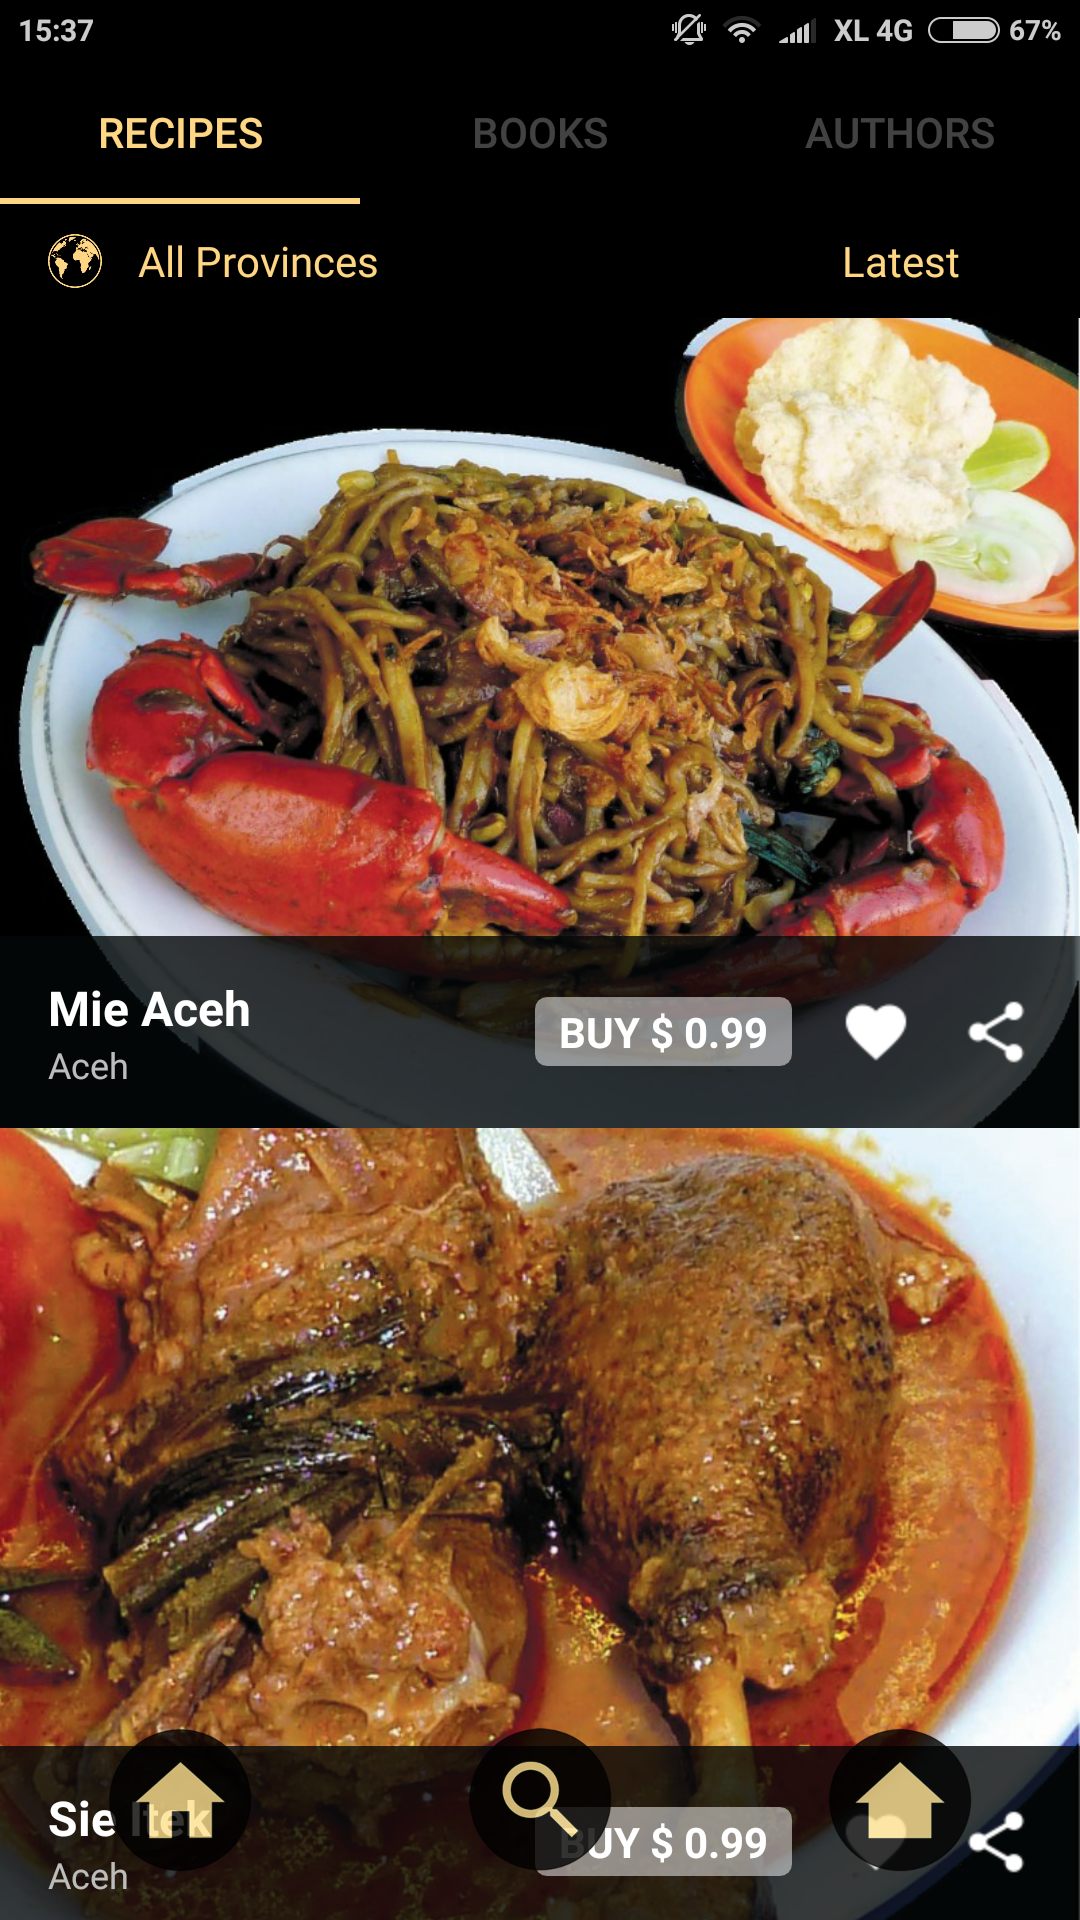
\includegraphics[width=0.3\textwidth]{gambar/kompas/utama}
	\caption{Halaman Utama Kompas Recipe}
\end{figure} 
\vspace{1cm}
Di dalam aplikasi tersebut terdapat kumpulan resep masakan yang dibagi menjadi dua jenis yaitu resep masakan berbayar dan resep masakan gratis. Terdapat banyak resep masakan yang menarik namun berbayar seperti Mie Aceh, Ayam Tangkap, dan Nasi Uduk. Untuk itu, penulis ingin mengembangkan aplikasi dengan resep masakan yang keseluruhannya gratis, sesuai dengan prinsip \textit{Open Source}.
\begin{figure}[H]
	\centering
	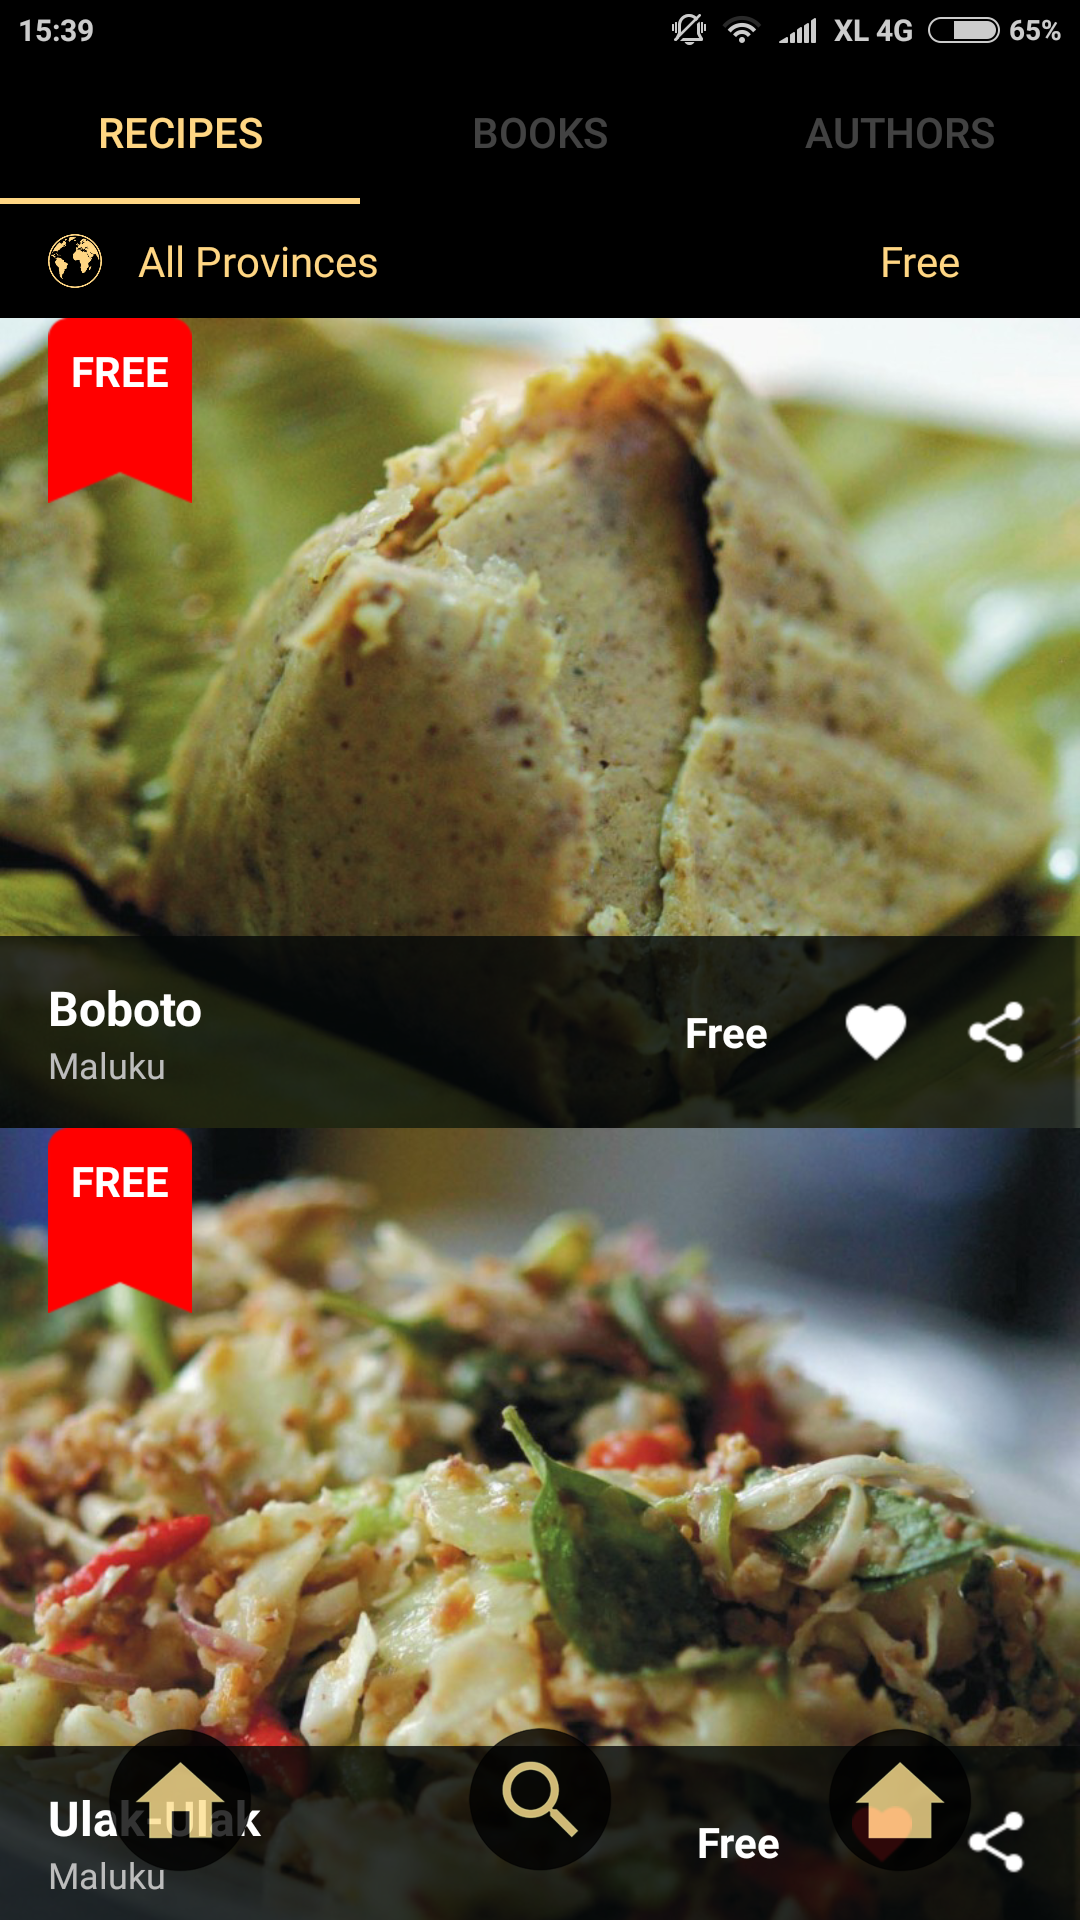
\includegraphics[width=0.3\textwidth]{gambar/kompas/free}
	\caption{Resep Masakan Gratis dari Kompas Recipe}
\end{figure} 
 Selain itu, Kompas Recipe tidak menyediakan video pembuatan makanan yang terdapat pada resep yang dibaca oleh pengguna. Aplikasi yang akan dibuat oleh penulis akan menyertakan video pembuatan makanan yang terdapat pada resep yang ada di dalam aplikasi tersebut. Penulis akan menamai aplikasi tersebut dengan nama Masak Yuk. Kata-kata tersebut sebenarnya merupakan ajakan bagi para masyarakat untuk memasak sendiri di rumah bersama keluarga, kerabat maupun teman-teman pengguna.


\section{Batasan Masalah}
Karena keterbatasan waktu, dana, tenaga, teori-teori dan supaya penelitian dapat dilakukan secara lebih mendalam maka tidak semua masalah akan diteliti. Berikut merupakan batasan-batasan yang diterapkan oleh peneliti
\begin{itemize}
	\item Peneliti akan membuat aplikasi tersebut dengan menggunakan \emph{software}  IDE (\emph{Integrated Development Environtment}) Android Studio. Peneliti memilih menggunakan Android Studio karena fiturnya yang sudah cukup lengkap dan sangat membantu dalam proses pembuatan aplikasi Android. Selain itu, kelengkapan API (\emph{Application Programming Interface}) dan banyaknya dukungan yang tersedia secara \emph{online} memudahkan peneliti dalam mengembangkan sebuah aplikasi Android.
	\item  Peneliti akan langsung menggunakan \emph{smartphone} berbasis Android dalam proses \emph{debugging} dan \emph{testing}. Versi android yang digunakan adalah Lollipop (Android 5.0) dengan API 21.
	\item Koneksi internet yang cepat, minimal pada kecepatan HSPA
	\item Banyaknya resep masakan yang akan dimasukkan kedalam aplikasi sejumlah 30 resep. Jumlah wishlist maksimal 3 resep.
	\item Uji coba hanya akan dilakukan oleh Ahli yang sudah berpartisipasi dalam proses identifikasi awal.
	\item Elemen-elemen yang akan diujikan pada uji coba ahli adalah konten, tampilan, dan fungsionalitas.
\end{itemize}
\vspace{1cm}
\section{Rumusan Masalah}
Rumusan masalah berdasarkan latar belakang di atas adalah:
\begin{enumerate}
	\item Bagaimanakah bentuk aplikasi resep masakan terintegrasi \emph{food channel} YouTube berbasis Android?
	\item Bagaimana cara mengembangkan aplikasi resep masakan terintegrasi \emph{food channel} YouTube berbasis Android?
	\item Bagaimana cara mengintegrasikan YouTube dengan aplikasi Android?
\end{enumerate}


\section{Tujuan Penelitian}
Tujuan dari penelitian ini adalah: 
\begin{enumerate}
	\item Untuk mengetahui bentuk atau wujud aplikasi resep masakan terintegrasi \emph{food channel} YouTube berbasis Android. 
	\item Untuk memaparkan fitur-fitur yang terdapat pada aplikasi tersebut. Selain itu, peneliti juga ingin menggali dan mengetahui cara mengembangkan aplikasi resep masakan terintegrasi food channel YouTube berbasis Android. 
	\item Untuk mengetahui lebih lanjut bagaimana cara mengintegrasikan YouTube, khususnya \emph{food channel} Youtube, dengan aplikasi Android. 
\end{enumerate}

\section{Manfaat Penelitian}
Penelitian ini memiliki banyak manfaat, yaitu: 
	\begin{enumerate}
		\item Bagi Penulis\\
		Melalui penulisan penelitian ini, penulis dapat memahami cara mengembangkan aplikasi Android secara baik dan benar serta mengetahui cara mengintegrasikan YouTube ke dalam sebuah aplikasi Android
		\item Bagi Program Studi Sistem Komputer\\
		Penulisan penelitian ini memberikan gambaran bagi seluruh mahasiswa khususnya bagig mahasiswa program studi Ilmu Komputer Universitas Negeri Jakarta tentang bagaimana cara mengembangkan suatu aplikasi Android yang tidak hanya bermanfaat bagi penulis saja tetapi juga bermanfaat untuk masyarakat dari berbagai kalangan, mulai dari anak-anak hingga orang dewasa yang ingin memasak dengan memanfaaatkan teknologi \emph{smartphone} Android sebagai referensi masakan mereka  
		\item Bagi Masyarakat\\
		Penelitian, termasuk aplikasi yag dibuat oleh penulis, dapat dimanfaatkan sebagai sumber referensi utama bagi masyarakat yang ingin memasak dan ingin memanfaatkan \emph{smartphone} sebagai media referensinya.  Menurut penulis, menggunaan \emph{smartphone} sebagai referensi memasak menggantikan buku resep adalah solusi praktis di era digital saat ini karena masyarakat tidak perlu lagi membeli buku atau membawa buku dalam jumlah yang banyak untuk memasak.		
	\end{enumerate}

\section{Jenis Penelitian}
Jenis Penelitian yang dijalani oleh Peneliti berjenis Rekayasa Produk. Jenis penelitian ini mengarahkan penulis kepada pengembangan sebuah sistem informasi berbasis aplikasi ponsel pintar \emph{smartphone}.		
% Baris ini digunakan untuk membantu dalam melakukan sitasi
% Karena diapit dengan comment, maka baris ini akan diabaikan
% oleh compiler LaTeX.
\begin{comment}
\bibliography{daftar-pustaka}
\end{comment}
